\clearpage
\newpage

\chapter{Results}
\label{cha:5}
\texttt{soweego} has been tested against the 19 September 2018 \texttt{MusicBrainz} dump\footnote{\url{ftp://ftp.eu.metabrainz.org/pub/musicbrainz/data/fullexport/}} and a sample of Wikidata entities.
The MusicBrainz artist subset contains \textbf{986,765 artists}\footnote{Entries in MusicBrainz tagged as artists or not tagged} and \textbf{181,221 aliases}. The Wikidata sample consists of \textbf{1100} entities randomly picked from 1\% of all musicians with no MusicBrainz link.\footnote{Entities having an \textit{occupation} property (\texttt{P106}) with value \textit{musician} (\texttt{Q639669}) and all its direct subclasses}
The table below shows the performance of the linking strategies outlined in Section~\ref{cha:42}.

\begin{table}[h]
    \centering
    \caption{Baseline linking strategies performance evaluation}
    \begin{tabular}{| l | c | c | c |}
        \hline
        \textbf{Strategy} & \textbf{Total matches} & \textbf{Checked} & \textbf{Precision} \\ \hline
        Perfect names & 381 & 38(10\%\%) & 84,2\%\\ \hline
        Perfect names + dates & 32 & 32 (100\%) & 100\%\\ \hline
        Normalized names & 227 & 24(10,6\%) & 70,8\%\\ \hline
        Perfect Link & 71 & 71(100\%) & 100\% \\ \hline
        Token Link & 102 & 102(100\%) & 99\%\\ \hline
    \end{tabular}
\end{table}

We first observe that link-based strategies achieve the best performance. They match almost 10\% of the sample with near 100\% precision. Figure~\ref{fig:linksvenn} illustrates why their coverage is 10\%: the \textit{perfect link matches} are a subset of the \textit{token link matches}.
We note that link-based strategies may be improved if we also consider the \texttt{official home page} Wikidata property, which has not been used so far.

The perfect name strategy improves recall with a 35\% coverage over the Wikidata sample, at the cost of precision. We assessed a randomly picked 10\% of these matches, obtaining a precision of 84\%. We argue that the relatively high precision stems from the very high quality of MusicBrainz data and the small size of the checked set.
We also isolated the subset of matches obtained by the perfect name strategy alone and not by other ones (cf. the leftmost set in Figure~\ref{fig:perfectsandtlinkvenn}), resulting in a precision of 68\%.\footnote{10\% of the leftmost set considered, 19 valid on 28 tests}

\begin{figure}[h]
  \begin{center}
   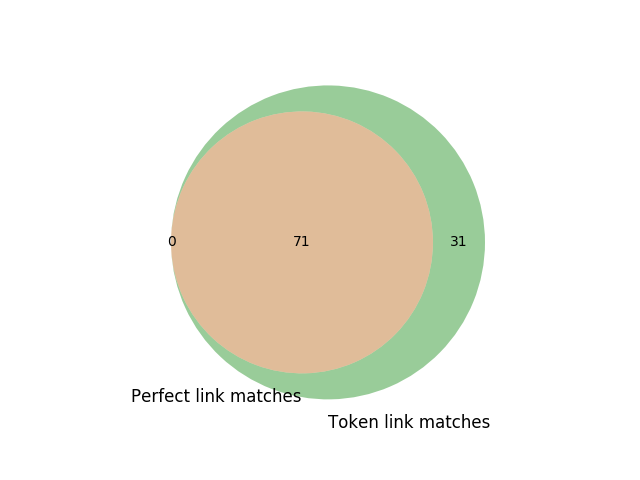
\includegraphics[height=200px]{images/plots/links.png}
   \captionof{figure}{Venn diagram of the links matches}
   \label{fig:linksvenn}
  \end{center}
\end{figure}

\begin{figure}[h]
  \begin{center}
   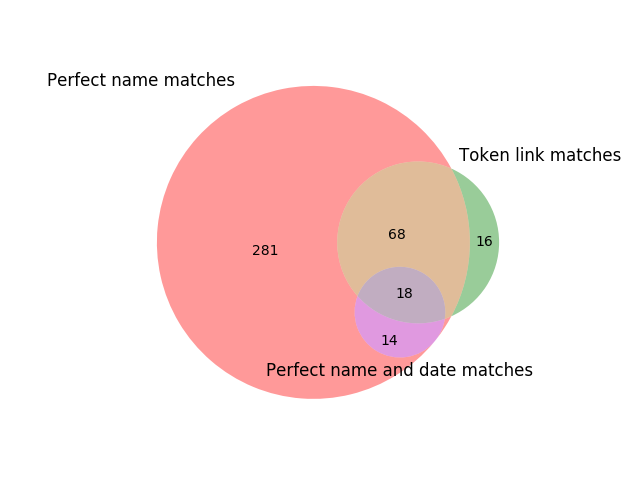
\includegraphics[height=200px]{images/plots/perfname_tlink_perfnamedate.png}
   \captionof{figure}{Venn diagram of perfect name matches, token link matches and perfect name and dates matches}
   \label{fig:perfectsandtlinkvenn}
  \end{center}
\end{figure}

The normalized name strategy performs similarly to the perfect name one. This is possibly due to the relatively big intersection of matches between the two strategies, as shown in Figure~\ref{fig:perfectandnormvenn}.
We notice that the normalized name strategy has a worse recall than the perfect name one. After further investigation, we realized that Wikidata multilingual labels are responsible for such performance decrease: the current implementation actually adds them to the token set of the entity and we trigger a match only if the source and target token sets are equal.
Hence, Arabic, Chinese, or Russian labels that are only available in Wikidata and not in MusicBrainz create a consistent amount of false negatives.

Unsurprisingly, date-based strategies yield high precision, although we note that they are not sufficient alone. Therefore, we can view them as constraints for other strategies, such as in the perfect name and dates one.

\begin{figure}[h]
  \begin{center}
   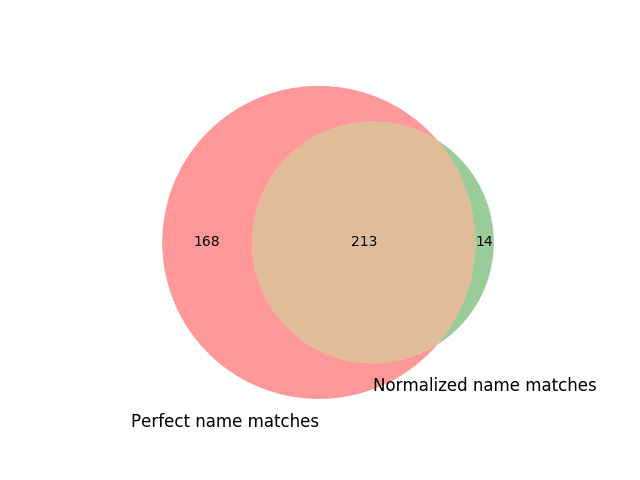
\includegraphics[height=200px]{images/plots/names.png}
   \captionof{figure}{Venn diagram of the perfect name matches and the normalized names matches}
   \label{fig:perfectandnormvenn}
  \end{center}
\end{figure}

